%http://texwelt.de/wissen/fragen/1774/wie-kann-ich-zahlen-%automatisch-in-zehnerpotenz-mit-siunitx-ausgegeben-lassen
\documentclass[11pt,ngerman,a4paper]{article}
%Gummi|061|=)
\usepackage{amsmath}
\usepackage{a4wide}
\usepackage{url}
\usepackage{amsthm}
\usepackage{amsbsy}
\usepackage{amssymb}
\usepackage[utf8]{inputenc}
\usepackage{rotating} 
\usepackage{here}
\usepackage{graphicx}
\usepackage{paralist}
\usepackage{selinput}
\usepackage[separate-uncertainty=true]{siunitx}
\usepackage{booktabs}
\sisetup{}
\SelectInputMappings{%
adieresis={ä},
germandbls={ß},
}
\title{\textbf{Versuch V503: Milikan-Versuch}}
\author{Martin Bieker\\
		Julian Surmann\\
		\\
		Durchgef\"{u}hrt am 03.06.2014\\
		TU Dortmund}
\date{}
\usepackage{graphicx}
\begin{document}
\renewcommand\tablename{Tabelle}
\renewcommand\figurename{Abbildung}
\maketitle
\thispagestyle{empty}
\newpage
\clearpage
\setcounter{page}{1}


\section{Einleitung}
In diesem Versuch soll die Elementarladung $e$ mit Hilfe der Öltröpfchenmethode nach Milikan bestimmt werden.
\section{Theorie}
Grundgedanke des hier beschrieben Versuchs ist die Bestimmung der Elementarladung durch Untersuchungen des Verhaltens von Öltropfen mit geringer Ladung im elektrischen Feld eines Kondensators. 
\subsection{Gravitation und Stokes-Reibung}
Zunächst werden die auf einen Tropfen wirkenden Kräfte bei abgeschalteten Feld untersucht. Einerseits wirkt die Differenz von Gravitations- und Auftriebskraft
\[
\vec F_g = -\frac43\pi r^3\left(\rho_{Oel}-\rho_{L}\right)\cdot \vec e_y
\]
Bewegt sich der Tropfen auf Grund dieser Kraft nach unten wirkt in entgegengesetzter Richtung die Reibungskraft $F_R$. Für die Reibung nach Stokes gilt:
\[
\vec F_R = 6\pi \eta_{L}rv \cdot \vec e_y
\]
Ist 
\begin{equation}
\vec F_G + \vec F_R = \vec 0
\label{gg0}
\end{equation}
hat sich die Gleichgewichtsgeschwindigkeit $v_0$  eingestellt. Aus Bedingung \ref{gg0} kann ein Zusammenhang für den Radius der Tröpfchen $r$ ermittelt werden:
\begin{equation}
r = \sqrt{\frac{9 \eta_L v_0}{2g\left(\rho_{Oel}-\rho_{L}\right)}}\mathrm{.}
\label{rv0}
\end{equation}
\subsection{Elektrische Kräfte auf geladene Teilchen} 
Befindet sich das Tröpfchen in einem elektrischen Feld und ist geladen, wirkt zusätzlich die elektrische Kraft
\[
\vec F_{el} = q\cdot \vec E \mathrm{.}
\]
Da das Feld durch einen Kondensator erzeugt wird gilt:
\[
\vec F_{el} = q\cdot \frac{U}{d} \cdot \vec e_y\mathrm{.}
\]
Dabei wird die Richtung der Kraft durch die Polung der Spannung am Kondensator bestimmt. Abbildung \ref{feldgg} zeigt die angreifenden Kräfte bei den verschiedenen Richtungen des Feldes mit den Gleichgewichtsgeschwindigkeiten $v_-$ und $v_+$. 
\begin{figure}[h]
\centering
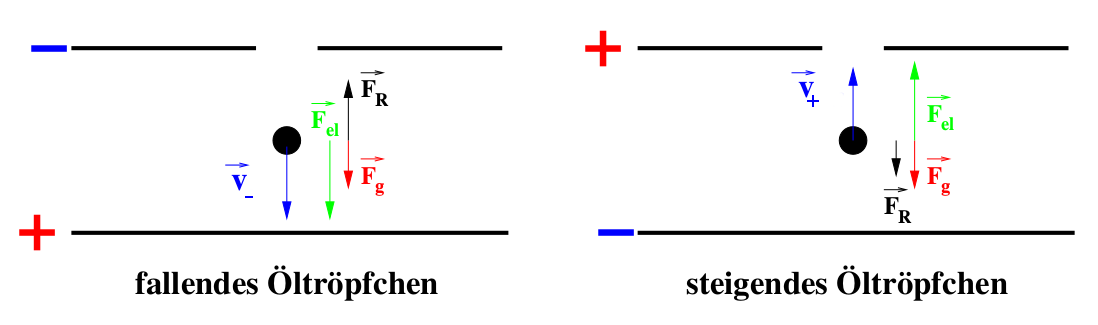
\includegraphics[scale=0.35]{abb1.png}
\caption{Kräftegleichgewichte bei verschiedenen Richtungen des elektrischen Feldes.[1]}
\label{feldgg}
\end{figure}
Aus dieser Grafik können folgende Kräftegleichgewichte abgelesen werden:
\begin{itemize}
\item Bei fallendem Tropfen ($v_-$):
\begin{equation}
\vec F_g+ \vec F_r - \vec F_{el}= \vec 0
\label{gg-}
\end{equation}

\item Bei steigendem Tropfen ($v_+$):
\begin{equation}
\vec F_g -\vec F_r +\vec F_{el}= \vec 0
\label{gg+}
\end{equation}
\end{itemize}
Mit diesen Gleichungen kann man Radius $r$ und Ladung $q$ der Tröpfchen berechnen. Es gilt:

\begin{equation}
r = \sqrt{\frac{9 \eta_L (v_--v_+)}{2g\left(\rho_{Oel}-\rho_{L}\right)}}\mathrm{.}
\label{r+-}
\end{equation}

\begin{equation}
q = 3\pi\eta_L\sqrt{\frac{9 \eta_L (v_--v_+)}{4g\left(\rho_{Oel}-\rho_{L}\right)}}\cdot \frac{(v_-+v_+)d}{U}
\label{q+-}
\end{equation}
Da die Tröpfchen auf Grund ihrer Größe das Reibungsgesetz von Stokes nicht erfüllen, muss bei der Berechnung die Viskosität korrigiert werden. Gemäß der Cunningham-Korrektur gilt:
\begin{equation}
q_{korr} = q_0 \left( 1+ \frac B{p\cdot r}\right)^{\frac32}
\end{equation}

\section{Aufbau}
Abblildung \ref{aufbau} zeigt den Aufbau der Versuchsapparatur.

\begin{figure}[htp]
\centering
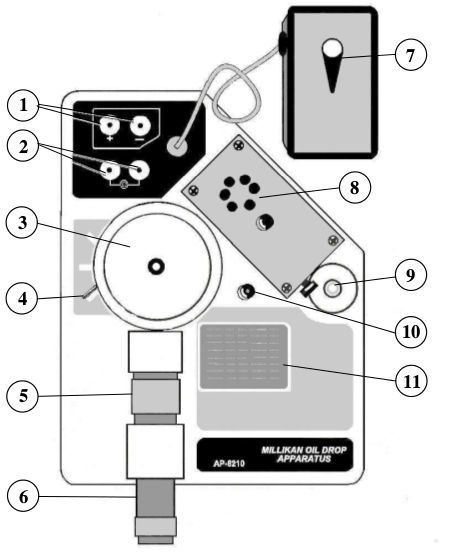
\includegraphics[scale=0.50]{abb2.png}
\caption{Schematischer Aufbau der Milikan-Apparatur.[1]}
\label{aufbau}
\end{figure}

\noindent
 In der Milikan-Kammer(3) befindet sich der Kondensator mit einem Plattenabstand von
\[
d = \SI{7.6250+-0.0051}{\milli\meter}
\]
Durch eine kleine Öffnung an der Oberseite der Kammer und in der oberen Kondensatorplatte können die Öltröpfchen in die Apparatur eingebracht werden. Diese Tropfen werden dann durch eine Lampe(8) angestrahlt und können so durch ein Mikroskop(5 \& 6) beobachtet werden. Zur einfacheren Versuchsdurchführung ist eine Kamera am Okular des Mikroskops befestigt. Diese überträgt die aufgenommenen Bilder an einen Monitor.Die Kondenstorspannung(1) wird durch ein Netzteil erzeugt und kann durch einen Schalter(7) eingeschaltet beziehungsweise umgepolt werden. 
Die Milikan-Kammer ist des Weiteren mit einem Koordinatengitter ausgestattet, um die von den Tröpfchen zurückgelegte Strecke zu messen. Der Abstand zwischen zwei Koordinatenlinien beträgt
\[
a = \SI{0.1}{\milli\meter}
\]
Da die Viskosität von Luft eine Funktion der Temperatur ist, befindet auch ein Thermowiderstand in der Kammer. Dieser kann mit Hilfe eines Multimeters (2) überwacht werden und ermöglicht somit die Messung der Temperatur innerhalb der Kammer. Unterhalb des Kondensators ist eine geringe Menge eines radioaktiven Präparats eingelassen, das mit einem Shutter(4) verschlossen ist. Wird dieser geöffnet kann durch den $\alpha$-Strahler die Luft in der Milikan-Kammer ionisiert werden. Auf diese Weise können weitere Ladungen auf die Öltropfen übertragen werden.
\section{Durchführung}
\subsection{Justierung}
Vor Beginn der Messung muss der Versuchsaufbau kalibriert werden. Hierzu wird zunächst die korrekte Ausrichtung der Milikan-Apparatur mit der am Gerät angebrachten Libelle(9) sichergestellt. Danach wird eine Kallibrations-Nadel in die Milikan-Kammer eingeführt. Hiermit kann sowohl die Tröpfchenebene, als das Koordinatengitter am Mikroskop scharf gestellt werden. Abschließend wird der Fokus und die Helligkeit so eingestellt, dass das innere der Kammer klar erkennbar ist.
\subsection{Messprogramm}
Zu Beginn der Messung wird die Kondensatorspannung auf 
\[
U_C = \SI{300}{\volt}
\]
eingestellt. Danach wird  eine geringe Menge Öl in die Kammer eingebracht. Nun wird auf dem Bildschirm ein geeignetes Tröpfchen gewählt. Dieses zeichnet sich durch eine geringe waagerechte Driftgeschwindigkeit und eine genügende Größe aus. An diesem Punkt muss sichergestellt werden, dass auf dem Tröpfchen Ladung befindet. Dies wird durch Anlegend und anschließendes Umpolen der Kondensatorspannung festgestellt. Ist keine Änderung der Bewegungsrichtung erkennbar, wird versucht, mit Hilfe eines $\alpha$-Strahlers, zusätzliche Ladung auf das Tröpfchen zu bringen. Ist dies nicht erfolgreich muss ein anderer Tropfen für die Messung gewählt werden.
Bei der eigentlichen Messung wird die Zeit $t$ messen, welche das Tröpfchen für eine Strecke
\[
s = \SI{0.5}{\milli\meter}
\]
benötigt. Für jeden Tropfen werden 3 Messungen durchgeführt. Die Laufzeiten werden ohne Kondensatorspannung $t_0$ und mit eingeschalteter Spannung in unterschiedlicher Polung $t_+$ und $t_-$ gemessen. Aus diesen Werten werden dann die Geschwindigkeiten
\[
v = \frac{s}{t}
\]
berechnet. Dieser Vorgang wird wiederholt, bis für 15 verschiedene Tropfen die 3 Geschwindigkeiten bekannt sind.

In einem zweiten Versuchsteil wird die Kondensatorspannung auf 
\[
U_C = \SI{150}{\volt}
\]
gesenkt. Für 15 weitere Tröpfchen werden die Laufzeiten bei eingeschalteter Spannung $t_+$ und $t_-$ bestimmt.
\section{Auswertung}
\subsection{Auswertung für $U=\SI{297}{\volt}$}
Die aufgenommenen Messwerte sind in Tabelle 1 abgebildet. In Tabelle 2 befinden sich die berechneten Ergebnisse und Zwischenergebnisse für alle Werte, bei denen
\begin{equation}
0.7 < \frac{v_{ab}-v_{auf}}{2 v_0} < 1.3
\end{equation}
gilt. Dadurch werden Werte aussortiert, bei denen sich die Ladung während der Beobachtung geändert hat.
\begin{table}[H]
\centering
\begin{tabular}{ccccc}
\toprule
$n$ &{$t_{Null}$[s]} &{ $t_{auf}$[s]} &{ $t_{ab}$[s]} &{ R[M$\Omega$] }\\
\midrule
1 &34.900 & 3.273 & 2.918 & 2.03\\
2 &58.948 & 5.011 & 7.655 & 2.01\\
3 &28.018 & 4.204 & 9.842 & 1.89\\
4 &15.755 & 7.946 & 4.245 & 1.89\\
5 &26.543 & 4.735 & 3.879 & 1.89\\
6 &23.904 & 5.640 & 3.685 & 1.85\\
7 &64.958 & 3.796 & 3.484 & 1.84\\
8 &26.536 & 11.756 & 6.005 & 1.84\\
9 &58.571 & 3.633 & 3.582 & 1.80\\
10 &61.098 & 20.798 & 14.684 & 1.80\\
11 &17.396 & 52.334 & 6.584 & 1.79\\
12 &27.842 & 5.237 & 3.838 & 1.79\\
13 &34.652 & 5.125 & 3.424 & 1.79\\
14 &47.401 & 3.125 & 2.967 & 1.77\\
15 &12.061 & 17.707 & 4.751 & 1.77\\
16 &55.808 & 9.272 & 7.093 & 1.77\\
17 &18.702 & 35.159 & 8.964 & 1.77\\
18 &37.240 & 5.758 & 4.510 & 1.77\\
19 &17.102 & 23.986 & 5.877 & 1.77\\
\bottomrule
\end{tabular}
\label{}
\caption{Messwerte mit $U=\SI{297}{\volt}$}
\end{table}

\begin{table}[H]

\sisetup{table-format = +3.2e+4}

\begin{tabular}{SSSSSSSS}
\toprule
$n$& $v_auf [\si{\meter\per\second}]$ & $v_ab [\si{\meter\per\second}]$&
$T [\si{\celsius}]$&
$\eta_L$ & 
$\eta_{eff}$&
$r[\si{\meter}]$ &
$q[\si{\coulomb}]$\\
\midrule
4 & 6.29e-05 & 1.18e-4 & 27.0 & 1.86e-05 & 1.68e-05 & 7.51e-07 & 3.7e-19\\
6& 8.87e-05 & 1.36e-4 & 28.0 & 1.86e-05 & 1.67e-05 & 6.97e-07 & 4.22e-19\\
7 & 1.32e-4 & 1.44e-4 & 28.0 & 1.86e-05 & 1.51e-05 & 3.49e-07 & 2.23e-19\\
8 & 4.25e-05 & 8.33e-05 & 28.0 & 1.86e-05 & 1.65e-05 & 6.48e-07 & 2.18e-19\\
11 & 9.55e-06 & 7.59e-05 & 29.0 & 1.87e-05 & 1.7e-05 & 8.29e-07 & 1.97e-19\\
12 & 9.55e-05 & 1.30e-4 & 29.0 & 1.87e-05 & 1.64e-05 & 6.00e-07 & 3.58e-19\\
15 & 2.82e-05 & 1.05e-4 & 30.0 & 1.87e-05 & 1.72e-05 & 8.94e-07 & 3.35e-19\\
16 & 5.39e-05 & 7.05e-05 & 30.0 & 1.87e-05 & 1.57e-05 & 4.14e-07 & 1.26e-19\\
17 & 1.42e-05 & 5.58e-05 & 30.0 & 1.87e-05 & 1.67e-05 & 6.57e-07 & 1.24e-19\\
18 & 8.68e-05 & 1.11e-4 & 30.0 & 1.87e-05 & 1.61e-05 & 4.99e-07 & 2.52e-19\\
19 & 2.08e-05 & 8.51e-05 & 30.0 & 1.87e-05 & 1.7e-05 & 8.16e-07 & 2.4e-19\\
\bottomrule
\end{tabular}
\label{}
\caption{Auswertung für $U=\SI{297}{\volt}$}
\end{table}
\noindent
Die Werte für die Vielfachen der Elementarladung sind grafisch in Abbildung \ref{plot1a} dargestellt.
\begin{figure}[h]
\hspace{-1.5cm}
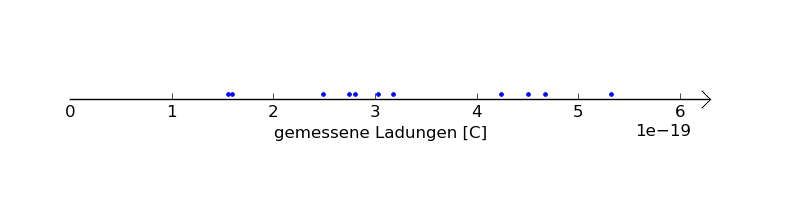
\includegraphics[scale=0.9]{plot1a.png}
\caption{Errechnete Ladungen bei $U=\SI{297}{\volt}$}
\label{plot1a}
\end{figure}
Die Werte lassen sich in drei Messwertgruppen aufteilen. Die erste Gruppe, bestehend aus zwei Messwerten, liegt bei ca. $\SI{1.6e-19}{\coulomb}$. Damit liegt sie Nahe an dem theoretischen Wert der Elementarladung von  $\SI{1.602e-19}{\coulomb}$. Die anderen Messwertgruppen müssten daher bei ca.  $\SI{3.2e-19}{\coulomb}$ und  $\SI{4.8e-19}{\coulomb}$ liegen. Leider sind die Abweichungen hier größer. Um einen sinnvollen Mittelwert bilden zu können, bräuchte es aufgrund der hohen Messfehler mehr Messwerte. 

\subsection{Auswertung für $U=\SI{150}{\volt}$}
Die aufgenommenen Messwerte sind in Tabelle 3 abgebildet. In Tabelle 4 befinden sich die berechneten Ergebnisse und Zwischenergebnisse für alle Werte. Da hier die Geschwindigkeit der Tröpfchen nicht ohne elektrisches Feld gemessen wurde, werden hier auch Messungen berücksichtigt, bei denen sich die Ladung des Tröpfchens verändert haben könnte.

\begin{table}[H]
\centering
\begin{tabular}{ccc}
\toprule
{ $t_{auf}$[s]} &{ $t_{ab}$[s]} &{ R[M$\Omega$] }\\
\midrule
23.776 & 20.512 & 1.76\\
27.441 & 9.432 & 1.76\\
24.321 & 16.568 & 1.76\\
27.289 & 16.873 & 1.76\\
21.155 & 18.188 & 1.76\\
40.118 & 8.290 & 1.76\\
24.523 & 8.476 & 1.76\\
7.059 & 5.758 & 1.76\\
10.672 & 4.887 & 1.75\\
13.574 & 6.956 & 1.75\\
5.253 & 3.278 & 1.75\\
8.079 & 10.210 & 1.75\\
13.310 & 5.877 & 1.75\\
3.606 & 3.904 & 1.75\\
6.833 & 3.876 & 1.75\\
\bottomrule
\end{tabular}
\label{}
\caption{Messwerte mit $U=\SI{150}{\volt}$}
\end{table}

\begin{table}[H]
\hspace{-1.cm}
\begin{tabular}{ccccccc}
\toprule
{$v_{auf}$[$10^{-5}$m/s]} &{ $v_{ab}$[$10^{-5}$m/s]} &{ T[$^\circ C$]} &{ $\eta_{L}[10^{-5}Nsm^{-2}]$} &{ $\eta[10^{-5}Nsm^{-2}]$} &{ r[$10^{-7}$m]} &{ q[$10^{-19}$C] }\\
\midrule
2.103 & 2.438 & 30.0 & 1.872 & 1.291 & 1.802 & 0.390\\
1.822 & 5.301 & 30.0 & 1.872 & 1.643 & 5.811 & 2.829\\
2.056 & 3.018 & 30.0 & 1.872 & 1.479 & 3.056 & 0.906\\
1.832 & 2.963 & 30.0 & 1.872 & 1.504 & 3.313 & 0.951\\
2.364 & 2.749 & 30.0 & 1.872 & 1.319 & 1.934 & 0.486\\
1.246 & 6.031 & 30.0 & 1.872 & 1.673 & 6.815 & 3.484\\
2.039 & 5.899 & 30.0 & 1.872 & 1.653 & 6.121 & 3.352\\
7.083 & 8.684 & 30.0 & 1.872 & 1.552 & 3.941 & 3.902\\
4.685 & 10.231 & 31.0 & 1.877 & 1.690 & 7.346 & 7.809\\
3.684 & 7.188 & 31.0 & 1.877 & 1.648 & 5.810 & 4.355\\
9.518 & 15.253 & 31.0 & 1.877 & 1.693 & 7.470 & 13.219\\
6.189 & 4.897 & 31.0 & 1.877 & nan & nan & nan\\
3.757 & 8.508 & 31.0 & 1.877 & 1.677 & 6.800 & 5.872\\
13.866 & 12.807 & 31.0 & 1.877 & nan & nan & nan\\
7.317 & 12.900 & 31.0 & 1.877 & 1.691 & 7.370 & 10.624\\
\bottomrule
\end{tabular}
\label{}
\caption{Auswertung für $U=\SI{150}{\volt}$}
\end{table}
\noindent
In Abbildung \ref{plot2a} sind die Ergebnisse graphisch dargestellt.
\begin{figure}[h]
\hspace{-1.5cm}
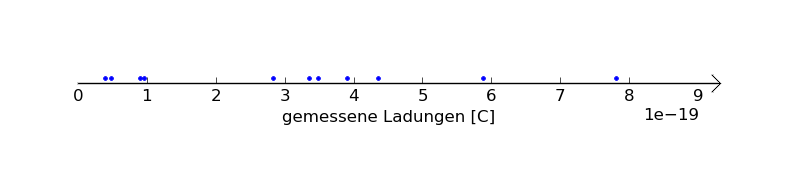
\includegraphics[scale=0.9]{plot2a.png}
\caption{Errechnete Ladungen bei $U=\SI{150}{\volt}$}
\label{plot2a}
\end{figure}
Hier ist keine Regelmäßigkeit zu erkennen, fehlerhafte Werte sind nicht von guten Werten zu unterscheiden. Außerdem liegen mehrere Werte unter dem Wert der Elementarladung.
\section{Diskussion}
An den Ergebnissen ist zu erkennen, dass eine genaue Messung geringer Ladungsmengen sehr schwer durchführbar ist. Die Fehler in den gemessenen Geschwindigkeiten wurden vor allem durch die relativ ungenaue manuelle Zeitmessung mit einer Stoppuhr verursacht. Des Weiteren wäre es für genauere Messwerte nötig gewesen, mit einzelnen Öltropfen mehrere Messungen durchzuführen, um einen Mittelwert mit einem statistischen Fehler zu bestimmen. Dies war auf Grund der kurzen Verweildauer der Tropfen in der Milikan-Kammer selten bis garnicht möglich.

\noindent
Die geringe Aussagekraft der zweiten Messreihe wird wahrscheinlich durch Öltröpfchen, die ihre Ladung während der Messung änderen, verursacht. Da die Gleichgewichtsgeschwindigkeit $v_0$ nicht gemessen wurde, können diese Tropfen nicht erkannt und verworfen werden. Dies führt bei der Auswertung zu fehlerhaften Ergebnissen.

\noindent
Es zeigt sich, dass für die genaue Bestimmung der Elemenentarladung
\[
q = \SI{1.602e-19}{\coulomb}
\]
eine sehr lange und sorgfältige Messung mit sehr vielen Messpunkten nötig wäre.
\section{Quellen}
\begin{enumerate}[{[}1{]}]
\item Entnommen der Praktikumsanleitung \textit{} der TU Dortmund. \\
Download am 04.06.14 unter:\\
 \url{http://129.217.224.2/HOMEPAGE/PHYSIKER/BACHELOR/AP/SKRIPT/Milikan.pdf}
\end{enumerate}
\section{Anhang}
\begin{itemize}
\item Auszug aus dem Messheft
\end{itemize}
\end{document}
